%\subsection{Performance test}
A performance test was developed to evaluate the users ability to operate a virtual prosthesis. The test was implemented as a 3D Fitts' Law target reaching test, similar to methods reported in \cite{Scheme2013, Scheme2013a}. The user controlled a circular cursor in a Cartesian coordinate system, where the cursor was to be matched with the appearing targets. Extension/flexion of the wrist moved the cursor horizontally, radial/ulnar deviation moved the cursor vertically and opened/closed hand increased/decreased the size of the cursor. The cursor moved proportional to contraction intensity with a velocity between 0 and 1, where 1 corresponded to the MVC. An illustration of the Fitts' Law test interface can be see in \figref{fig:fittsLawTask}. \\
To reach a target the user had to match the size and position and dwell within the area for 1 second. The target would appear for 15 seconds or until it was reached, after which a new target would appear and the cursor position would be reset to origin. A total of 16 targets would appear before the test ended. The sequence of targets appearing was different between all four test session, to avoid bias of subjects remembering the sequence in which targets would appear. \\


\vspace{-0.2cm}
Originally the Fitts' Law test had a single performance measure, \textit{throughput} (TP) \cite{Fitts1954}. TP uses the relationship between time taken to reach a certain target in seconds ($MT$) and the index of difficulty (ID), and is defined as:
%\vspace{-0.1cm}
\begin{equation} \label{eq:TP}
TP=\frac{1}{N}\sum_{i=1}^{N} \frac{ID_i}{MT_i} 
\end{equation}
%\vspace{-0.1cm}
\noindent Where $i$ is a specific movement and $N$ is the total number of movements. ID relates to the target's width $W$ and distance $D$ from origin, where $W$ and $D$ are unitless. The ID is calculated as: 
%\vspace{-0.1cm}
\begin{equation} \label{eq:ID}
ID=log_2(\frac{D}{W}+1)
\end{equation}
%\vspace{-0.1cm}
\noindent According to \cite{Scheme2013a}, it is in practice most resourceful to use a variety of ID's in a Fitts' Law test. Based on this assumption, the target ID's seen in \tabref{tab:P:ID} were calculated for this study.
\begin{figure}[H] 
	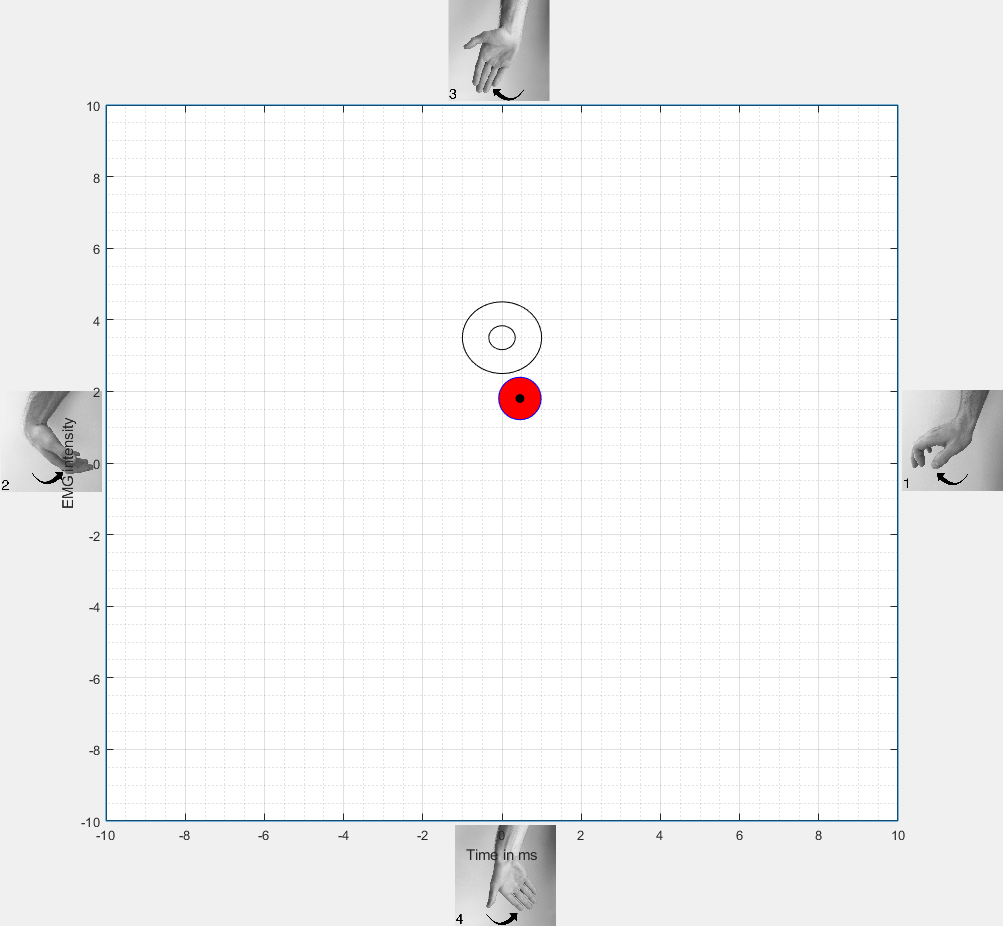
\includegraphics[width=0.49\textwidth]{figures/xBackground/perftestGUI}
	\caption{The implemented interface for the modified Fitts' Law test. The user controlled the red cursor with the centred bold mark. The target consisted of a circle with a larger circle surrounding it. The user was instructed in matching the cursor with the target, where the bold mark should be positioned inside the inner circle of the target, and the outer circle of the cursor should be matched in size with the outer circle of the target. The cursor would then turn green to indicate the matching was correct, and blue when the dwell time was reached.}
	\label{fig:fittsLawTask}
\end{figure}
%\vspace{-1.0cm}
Further performance measures were included similar to previously reported in \cite{Scheme2013, Scheme2013a}. These measures consists of \textit{Path Efficiency}, \textit{Overshoot}, \textit{Stopping Distance} and \textit{Completion Rate}. \\
The additional four measures were added to quantitatively assess performance of naturalness, spontaneity, and compensatory motions during control. The calculation of these features can be found in the appendix. 
\begin{table}[H]
	\centering
	\caption{The index of difficulty used in the Fitts' Law test.}
	\label{tab:P:ID}
	\begin{tabular}{lll}
		
		Distance		 & Width	         & ID				   \\ \hline \hline
		28.0     & 0.33 & 6.41                \\ %\hline \hline
		24.5     & 0.33 & 6.22                \\ %\hline
		22.0     & 0.33 & 6.01                \\ %\hline
		18.5     & 0.33 & 5.82                \\ %\hline
		16.0     & 0.33 & 5.61                \\ %\hline
		13.0     & 0.33 & 5.32                \\ %\hline
		12.5     & 0.33 & 5.27                \\ %\hline
		9.5      & 0.33 & 4.88                \\ \hline \hline
	\end{tabular}
\end{table}
